%%%%%%%%%%%%%%%%%%%%%%%%%%%%%%%%%%%%%%%%%%%%%%%%%%%%%%%%
%%%%%%%%%%%%%%%%%%%%%%%%%%%%%%%%%%%%%%%%%%%%%%%%%%%%%%%%
%%			            Capitulo 2					  %%
%%%%%%%%%%%%%%%%%%%%%%%%%%%%%%%%%%%%%%%%%%%%%%%%%%%%%%%%
%%%%%%%%%%%%%%%%%%%%%%%%%%%%%%%%%%%%%%%%%%%%%%%%%%%%%%%%
\chapter{Conceptos teóricos} \label{cap2}

En este capítulo se exponen los conceptos básicos y teóricos que otorgan la base teórica suficiente para la comprensión del funcionamiento de cada una de las funciones que desempeña cada programa (objetivos secundarios) que constituyen la parte de software del proyecto.

\newpage



%%%%%%%%%%%%%%%%%%%%%%%%%%%%%%%%%%%%%%%%%%%%%%%%%%%%%%%
%		            	Seccion          			  %
%%%%%%%%%%%%%%%%%%%%%%%%%%%%%%%%%%%%%%%%%%%%%%%%%%%%%%%
\section{Captura de eventos de dispositivos USB de interfaz humana} \label{s2_1}

%%%%%%%%%%%%%%%%%%%%% Subsección %%%%%%%%%%%%%%%%%%%%%
\subsection{Dispositivos de interfaz humana o ``HID Devices''} \label{s2_1_1}

Los dispositivos de interfaz humana o ``Human Interface Devices'' de donde proceden sus siglas HID, son dispositivos periféricos que permiten establecer comunicación entre el usuario humano y el computador siendo el primero el que toma el control del mismo. El computador recibe a su entrada datos de control introducidos por el usuario como pulsaciones de teclas y movimientos de ratón o de joysticks. Estos datos son llamados ``eventos'' y son procesados por el computador dando lugar a una respuesta que se visualiza a través de la pantalla. 

Aquellos dispositivos HID que se comuniquen con el computador utilizando el protocolo ``Universal Serial Bus'' o comúnmente llamado ``USB'' son denominados USB-HID Devices, o dispositivos USB de interfaz humana. 

En este proyecto, son necesarios dos dispositivos HID USB, el teclado y el ratón, que van a permitir al usuario tomar el control de dos equipos distintos. Además, también se hace uso de otro periférico como es una cámara para capturar el rostro y reconocer la posición de los ojos. Todos ellos se conectan a Raspberry Pi que funciona de idéntica forma a un computador, actuando como servidor o ``host'' de la comunicación mientras que todos estos periféricos cumplen la función de clientes o ```clients''. Cuando se pulsa una tecla o se realiza un movimiento con el ratón, Raspberry Pi recibe los datos introducidos por el humano y y devuelve una respuesta a los dispositivos HID. Todo esto, se hace posible mediante un conjunto de comandos o drivers que se ejecutan para permitir la comunicación entre los dispositivos y el servidor. Los drivers HID otorgan la capacidad al sistema operativo y a otro tipo de aplicaciones de acceder al cualquier hardware independientemente del fabricante sin conocer en profundidad sus características concretas, es decir, es el intermediario entre el hardware y el sistema operativo.



%%%%%%%%%%%%%%%%%%%%% Subsección %%%%%%%%%%%%%%%%%%%%%
\subsection{Disparadores y manejadores de eventos} \label{s2_1_2}

Los dispositivos HID intercambian datos con el servidor usando un conjunto de datos denominados ``reports'' que pueden albergar varios tipos de datos y son de un tamaño fijo. Los drivers permiten que el sistema operativo lea los ``reports'' y son los manejadores los que permiten a los programas interactuar con los drivers. Por otro lado, los drivers proporcionan interfaces de entrada/salida que posibilitan la comunicación dispositivo-servidor. La interfaz encargada de la comunicación con dispositivos USB HID es leída por la aplicación como un archivo, de esta forma se obtiene la ruta del mismo trabajando con su correspondiente descriptor sobre el cual se pueden realizar operaciones de lectura y escritura. 

La función que cumplen los manejadores es despachar aquellos eventos recibidos por los dispositivos HID. Antes de que el manejador opere con los datos que recibe, un disparador analiza los eventos y determina su tipo para enviarlo al manejador adecuado\footnote{Para mejor comprensión, acúdase a la sección 3.1.}. Puede suceder que el disparador se tope con un evento extraño para el cual no existe un manejador. En ese caso, el disparador eleva una excepción y rechaza el evento, de ahí, el uso de excepciones\footnote{Véase la sección 2.1.4.}.

\begin{figure}
\centering
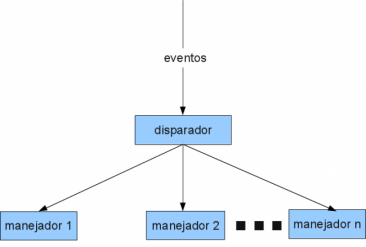
\includegraphics[scale = 0.7]{capitulo_02/figuras_dir/disparador.jpg}
\caption{Diagrama de manejadores. Imagen tomada de Genbeta:dev - Introducción a la programación dirigida por eventos: https://www.genbetadev.com/paradigmas-de-programacion/introduccion-a-la-programacion-dirigida-por-eventos}
%\label{fig:figura4}
\end{figure}

%%%%%%%%%%%%%%%%%%%%% Subsección %%%%%%%%%%%%%%%%%%%%%
\subsection{Sistema Linux} \label{s2_1_3}

%/////////////////// Subsubsección ///////////////////%
\subsubsection{Drivers de los dispositivos}\label{s2_1_3_1}

Existe un fichero en los sistemas Linux que constituye una parte del driver de los dispositivos HID que permite la comunicación entre las aplicaciones desarrolladas para capturar eventos de estos dispositivos. Se trata de ``Hidraw'', una interfaz de dispositivos bluetooth y USB HID cuyo uso es independiente a tipo de hardware utilizado. Mediante ``Hidraw'' se pueden obtener los eventos deseados sin formato, tal y como son enviados por el dispositivo. 

El sistema operativo interacciona con ``Hidraw'' como si se tratase de un archivo, de hecho, puede visualizarse en la ruta {\itshape/dev/hidraw}. Como ya se ha mencionado, las aplicaciones se comunican con el hardware interactuando con el driver que es el que proporciona la interfaz de entrada y salida. La forma de hacerlo consiste en realizar una llamada al sistema de apertura mediante la función {\itshape open()\footnote{Este concepto se introduce en la sección 2.8.1}} y así obtener el descriptor del archivo con el que se realiza la lectura con {\itshape read()\footnote{Este concepto se introduce en la sección 2.8.1}} para obtener los eventos.\footnote{Véase el capítulo 3}

%/////////////////// Subsubsección ///////////////////%
\subsubsection{Descriptores de archivo}\label{s2_1_3_2}

Cuando se realiza una llamada al sistema con la función {\itshape open()} de un archivo como por ejemplo, en el caso anterior, con ``Hidraw'', la función devuelve un número entero que constituye el descriptor de archivo. Si la apertura no ha sido errónea, ese número es distinto a ``-1''. Este descriptor se define como un enlace o puntero al archivo sobre el que se ha realizado la operación de forma que aquellas que se realicen con el descriptor, actúan directamente sobre el archivo.

%%%%%%%%%%%%%%%%%%%%% Subsección %%%%%%%%%%%%%%%%%%%%%
\subsection{Excepciones en C} \label{s2_1_4}

La finalidad de la excepciones es tratar los errores de alguna forma. Hay errores de los cuales se tiene información para poder tratarlos y otros en los que no. Con el lenguaje C se pueden usar excepciones mediante la librería ``exception.h'', de hecho, se emplea en ``reactor'', una biblioteca altamente usada en este proyecto para manejar eventos, de la cual se habla en las próximas secciones. Aprovechando la propiedad de la programación orientada a objetos de C\footnote{Véase la sección 2.1.5}, las excepciones se declaran en una estructura como la siguiente: 
\begin{listing}
\begin{minted}[bgcolor=bg,
               frame=lines,
               framesep=2mm,
               linenos]
               {C}
typedef struct {
    int error_code;
    const char* what;
} exception;

define_exception_type(exception);
\end{minted}
\caption{Excepción como un objeto}
%\label{Listing}
\end{listing}

El código de error es un número entero y la variable ``what'' apunta a una cadena de texto que informa sobre el error.
La forma de tratar las excepciones se muestra en ``Listing \ref{Lis: tratamiento}''.
\begin{listing}
\begin{minted}[bgcolor=bg,
               frame=lines,
               framesep=2mm,
               linenos]
               {C}
try{
    ...
}
catch (ex){
    ...
}
\end{minted}
\caption{Tratamiento de excepciones}
\label{Lis: tratamiento}
\end{listing}


Donde ``ex'' es la excepción de tipo ``exception'' definida en la estructura anterior. Cuando ``catch'' detecta una excepción es porque en ``try'' se ha producido una elevación de excepción en la ejecución normal del código. En ese momento, se interrumpe el proceso y ``catch'' trata el error que ha producido el lanzamiento de la excepción. En este caso, si ``catch'' sabe cómo tratar el error o ya se conoce el tipo de error que se ha producido, puede ejecutar el código correspondiente o incluso informar por pantalla sobre el mismo, en caso contrario, puede lanzar de nuevo otra excepción \citep[pág. 87--89]{tallerRPi}.

Cuando se produce un error, la forma de lanzar una excepción se representa en ``Listing \ref{Lis: Lanzamiento}''.

\begin{listing}
\begin{minted}[bgcolor=bg,
               frame=lines,
               framesep=2mm,
               linenos]
               {C}
if (funcion<0)
throw ex;
\end{minted}
\caption{Lanzamiento de una excepción}
\label{Lis: Lanzamiento}
\end{listing}

Sin embargo, si se elevan excepciones antes de que se haga una llamada a las funciones de liberación de memoria\footnote{Función free() para liberar memoria después de haberla reservado con malloc().} o de cierre de archivos\footnote{Función close() para cerrar un archivo tras haberlo abierto con open().} sin ejecutarse, se quedan recursos en memoria dinámica sin liberar. Para evitarlo, las excepciones deben lanzarse después de estas funciones.

%%%%%%%%%%%%%%%%%%%%% Subsección %%%%%%%%%%%%%%%%%%%%%
\subsection{Programación orientada a objetos} \label{s2_1_5}

Se trata de un mecanismo de programación que usa objetos como pueden ser números enteros, números fraccionales, caracteres, etc. El lenguaje C dispone de este mecanismo y por tanto, se pueden crear estructuras de datos que definen objetos concretos. Estos objetos están constituidos por los llamados ``atributos del objeto'' que son datos que caracterizan o definen al objeto. En la bliblioteca ``Reactor'' se hace uso de esta funcionalidad (``Listing \ref{Lis: Objeto reactor}'').

\begin{listing}
\begin{minted}[bgcolor=bg,
               frame=lines,
               framesep=2mm,
               linenos]
               {C}
typedef struct reactor_reactor;
typedef void (*reactor_function)(reactor* r);
typedef void (*reactor_exception_function)(reactor* r, exception e);
    
struct reactor_{
    int running;
    int paused;
    int max_fd;
    fd_set fds;
    int num_handler* handlers[REACTOR_MAX_HANDLERS];
    struct timeval tv, timeout;
    reactor_function destroy;
    reactor_exception_function exception;
};
\end{minted}
\caption{Objeto ``reactor''}
\label{Lis: Objeto reactor}
\end{listing}


El código anterior define un objeto denominado ``reactor'' a través de una estructura que contiene distintos datos o atributos. A esta definición se le llama ``clase''. Una vez especificado el objeto, éste debe construirse. Existen dos funciones llamadas ``constructores'' \citep[pág. 93--95]{tallerRPi}: ``reactor\_new()'' y ``reactor\_init()''. El primero, se encarga de reservar memoria para un objeto de tipo ``reactor'', llamar a la función ``reactor\_init()'', crear un puntero a una función que libera la memoria y devolver un puntero a una estructura de tipo ``reactor'' (``Listing \ref{Lis: constructor}''). 


\begin{listing}
\begin{minted}[bgcolor=bg,
               frame=lines,
               framesep=2mm,
               linenos]
               {C}
reactor* reactor_new()
{
    reactor* r= malloc(sizeof(reactor));
    reactor_init(r);
    r->destroy=reactor_destroy_and_free;
    return n;
}
\end{minted}
\caption{Constructor del objeto ``reactor''}
\label{Lis: constructor}
\end{listing}


La segunda función se encarga de asignar valores a los atributos del objeto (``Listing \ref{Lis: inicializacion}''). Además, también genera un puntero a una función, el cual debe apuntar a la función adecuada. Esta función se denomina ``función virtual'' y se encarga de liberar todos aquellos elementos de ``reactor'' reservados en la memoria. Debido a esto, esta función también es conocida como ``destructor virtual'' \citep[pág. 93--95]{tallerRPi}.


\begin{listing}
\begin{minted}[bgcolor=bg,
               frame=lines,
               framesep=2mm,
               linenos]
               {C}
void reactor_init(reactor* r)
{
    r->running = r->paused = 0;
    FD_ZERO(&r->fds);
    r->max_fd = -1;
    r->num_handlers = 0;
    r->destroy = reactor_destroy_members;
    r->exception = default_exception;
    reactor_set_default_timeout(r);
}
\end{minted}
\caption{Inicialización de los atributos del objeto ``reactor''}
\label{Lis: inicializacion}
\end{listing}

    
Hasta ahora, solo se conoce la relevancia de la programación orientada a objetos en el desarrollo de la biblioteca ``Reactor''. En el próximo capítulo se estudia la importancia que tiene el objeto ``reactor'' así como un objeto más, ``event\_handler'', en el manejo de eventos.
    
%%%%%%%%%%%%%%%%%%%%% Subsección %%%%%%%%%%%%%%%%%%%%%
\subsection{Biblioteca ``Reactor''}\label{s2_1_6}

La biblioteca reactor implementa un patrón de programación basado en programación orientada a objetos que permite elaborar programas con una arquitectura que otorga cierto orden a la aplicación que se desarrolla. Su función consiste en modelar los datos entrantes al sistema como eventos, de esta forma, ``Reactor'' dispone de varios tipos de manejadores, cada uno de ellos sirve para un tipo de evento concreto. En el caso de este proyecto, el manejador apropiado para eventos de dispositivos HID es el llamado ``event\_handler'' que se encarga de procesar eventos de tipo ``handle''\footnote{Véase el capítulo 3}. Por otro lado, ``socket\_handler'' es el manejador usado en la comunicación en red entre Raspberry Pi y Arduino. 

Los objetos ``reactor'' y ``event\_handler'' usados en esta biblioteca cumplen distintas funciones. Los manejadores se implementan con objetos de tipo ``event\_handler'' y los objetos de tipo ``reactor'' contienen todos los datos necesarios para permitir la demultiplexación de los eventos, es decir, actúa como disparador eligiendo el tipo de manejador apropiado para los eventos de entrada \citep[pág. 97--100]{tallerRPi}.

La finalidad de esta biblioteca es tanto facilitar el manejo de eventos de varios tipos como fomentar la implementación de programas legibles y sin falsa apariencia de correcto funcionamiento como sucede aquellas veces en las que los programas se desarrollan sin seguir un patrón concreto, complicándose estrepitósamente.













\newpage
%%%%%%%%%%%%%%%%%%%%%%%%%%%%%%%%%%%%%%%%%%%%%%%%%%%%%%%
%		            	Seccion          			  %
%%%%%%%%%%%%%%%%%%%%%%%%%%%%%%%%%%%%%%%%%%%%%%%%%%%%%%%
\section{Seguimiento ocular} \label{s2_2}

%%%%%%%%%%%%%%%%%%%%% Subsección %%%%%%%%%%%%%%%%%%%%%
\subsection{Biblioteca openCV} \label{s2_2_1}

OpenCV es una biblioteca que, tal y como su nombre indica, proporciona código abierto de visión computacional (Open Source Computer Vision Library). Se utiliza para aplicaciones que se ejecutan en tiempo real, por tanto, ofrece una gran eficiencia a nivel computacional procesando y analizando imágenes, estructuras de datos y muchas tareas que requieren potencia de procesamiento. De hecho, OpenCV ha sido desarrollado debido al crecimiento de algoritmos de visión computacional que evidencian la necesidad de conseguir software más sofisticado y de mayor velocidad. 
Esta herramienta se caracteriza por su versatilidad, permitiendo al usuario su uso en diferentes entornos de programación como C++, Python, Matlab, Ruby y Java. Asimismo, se puede usar en multitud de sistemas operativos, tales como Windows, Linux, MacOs, iOs e incluso Android y su implementación está basada en C y C++ optimizado.

\begin{figure}
\centering

\includegraphics[scale = 0.5]{capitulo_02/figuras_dir/OpenCV.jpg}
\caption{Logotipo de OpenCV}
%\label{fig:figura2}
\end{figure}

OpenCV cuenta con una estructura interna particular, es decir, consta de cinco partes distintas \citep{libroopencv}:
\begin{itemize}
\item CV: Procesamiento básico de imágenes de alto nivel y algoritmos de visión computacional.
\item MILL: Incluye la mayoría de clasificadores y herramientas.
\item HihgGUI: Rutinas de entrada/salida y funciones para almacenar y cargar vídeo e imágenes.
\item CXCORE: Estructuras básicas de datos.
\item CvAux: Algoritmos experimentales.
\end{itemize}

\begin{figure}
\centering
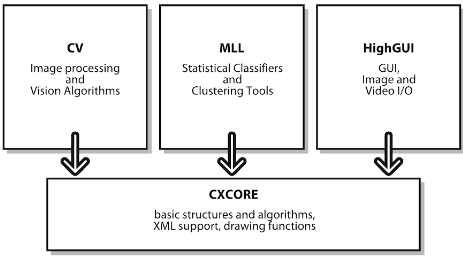
\includegraphics[scale = 0.7]{capitulo_02/figuras_dir/estructura.jpg}
\caption{Estructura básica de OpenCV. Imagen tomada del libro ``Learning OpenCV: Computer Vision with the OpenCV Library'' - OpenCV Structure and Content, página 13}
\label{fig:figura3}
\end{figure}

Esta estructura otorga a la totalidad de la biblioteca un gran cantidad de funciones que permiten solucionar casi todos los problemas de visión computacional \citep{arevalo2004libreria}. 

OpenCV contiene ocho módulos. Cada una de ellos tiene unas características y funciones diferentes:
\begin{itemize}
\item {\bfseries\itshape core}: Contiene funciones aritméticas, estructuras de datos elementales y funciones empleadas por otros módulos.
\item {\bfseries\itshape imgproc}: Contiene las funciones de procesamiento de imágenes.
\item {\bfseries\itshape video}: Permite la realización de la estimación de movimiento de objetos y la sustracción de fondo de la imagen. Además, contiene algoritmos de seguimiento de objetos.
\item {\bfseries\itshape calib3d}: Permite la calibración de la cámara y aporta elementos de reconstrucción 3D.
\item {\bfseries\itshape features2d}: Contiene funciones de detección de puntos y descriptores.
\item {\bfseries\itshape objdetect}: Permite la detección distintos tipos de objetos.
\item {\bfseries\itshape highgui}: Contiene las funciones de lectura y escritura de vídeos, imágenes, capturas y de interfaz de usuario.
\item {\bfseries\itshape gpu}: Proporciona algoritmos acelerados por GPU.
\end{itemize}

El propósito de esta biblioteca en este proyecto es de detectar la posición de los ojos para determinar el lugar hacia el que mira el observador y así poder mandar los eventos de teclado y ratón a un computador u otro. OpenCV permite esto y otras muchas mas funciones además de presentar ciertas ventajas que determinan su elección para esta aplicación. Algunas de ellas son \citep{arevalo2004libreria}:
\begin{itemize}
\item Disposición de un gran número de funciones: operaciones con estructuras matemáticas básicas, reconocimiento de patrones, operaciones estadísticas, calibración de cámaras, reconocimiento de gestos, determinación de posiciones, seguimiento de objetos, etc. 
\item Es software libre.
\item Proporciona herramientas de alto nivel. Puede ser usando tanto en el entorno académico como en el entorno profesional. 
\item Es gratuito.
\item Es rápido y estable.
\item Existe una gran comunidad de desarrollo así como tutoriales y demás contenidos formativos.
\item Proporciona un amplio abanico de herramientas a diferencia de otros paquetes de su mismo propósito sean o no de código libre.
\item No es necesario hardware específico, es decir, es compatible con casi todas las cámaras comerciales.
\item Contiene bibliotecas de datos estadísticos.
\end{itemize}


%/////////////////// Subsubsección ///////////////////%
\subsubsection{Clasificadores}\label{s2_2_1_1}

Los clasificadores intervienen en el reconocimiento de determinados objetos, en función de la finalidad para la cual han sido creados. Existen varios tipos de clasificadores suministrados por la biblioteca que permiten la detección de caras, ojos y otro tipo de objetos.
 A parte de los ya existentes, los clasificadores también pueden crearse y ``entrenarse'' para conseguir el reconocimiento del objeto que se desea. Para el entrenamiento de un clasificador empleando un conjunto de muestras se usa el denominado algoritmo ``boosting''. Este algoritmo crea clasificadores que determinan la región de la imagen en la que se encuentra el objeto. Estos clasificadores después se organizan en cascada y de esta forma, incrementar la eficiencia en la detección.

En el caso de este proyecto, interesa conocer los eventos de la posición de los ojos, para ello, en primer lugar es necesario detectar la posición de la cara, y dentro de esta región, detectar la posición de los ojos. Una vez conocida la región que contiene los ojos, de la misma forma se puede conocer la posición del iris. Para esto, se emplean clasificadores que están implementados con el algoritmo de Viola-Jones. Este algoritmo es usado en la detección de rostros y se caracteriza por su eficiencia y su baja tasa de errores en la detección a diferencia de otro tipo del algoritmos que se pueden encontrar en la actualidad. El método se emplea para reconocer un rostro en una imagen. En primer lugar, el algoritmo requiere imágenes con cara (denominadas imágenes positivas) e imágenes sin cara (denominadas imágenes negativas) para poder entrenar al clasificador. De esas imágenes se obtienen las características comunes a todas las caras.
Las características comunes que presenta un rostro son \citep{iglesias2016reconocimiento}:
\begin{itemize}
\item La zona de los ojos es mas oscura en relación a la zona de las mejillas
\item La zona del puente nasal es mas claro que la región de los ojos. 
\end{itemize}

Para reconocer en cada imagen el rostro, se desliza una máscara sobre la imagen y se realiza la suma de los valores de los píxeles bajo el área blanca y se resta con el valor de la suma de los píxeles bajo el área negra. A estas máscaras se les denomina ``Haar-like features''. Como resultado, se obtiene una característica que representa esa región. Hay varios tipos de máscaras y cada una de ellas está vinculada a un clasificador, es decir, cada clasificador deriva de una variante de ``feature'' o característica. Hay tres tipos de máscaras: de dos, tres y cuatro regiones rectangulares, sin embargo, este algoritmo usa solamente el de dos y tres regiones. 

\begin{figure}
\centering
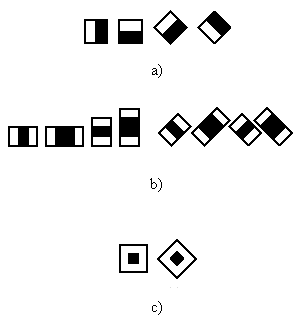
\includegraphics[scale = 0.7]{capitulo_02/figuras_dir/mascaras.jpg}
\caption{Algunos tipos de ``Haar-like features''}
%\label{fig:figura4}
\end{figure}

A través de cada clasificador, se toman todas las características de rostro dentro y fuera de la máscara y se clasifican como zonas positivas (con cara) o negativas (sin cara) en cada imagen de entrenamiento. Esto quiere decir que el algoritmo busca combinaciones de ``Haar-like features'' \citep{opencvhaar} que uniéndolos tomen una forma aproximada a la del rostro que se analiza en la imagen. Estas regiones se clasifican atendiendo a las características comunes que presentan los rostros. Evidentemente, cuanto mayor sea el número de características detectadas mayor será la precisión obtenida en la clasificación. Sin embargo, siempre hay clasificaciones erróneas pero se escoge aquella área clasificada que presente un índice mínimo de error. Tras cada clasificación, el peso de las regiones mal clasificadas se reduce y aumenta el peso de las que están bien clasificadas. Este proceso se realiza mediante el algoritmo de Adaboost \citep{opencvorg}. Después de cada proceso de clasificación se calculan nuevas tasas de error hasta que el sistema toma mayor precisión en la detección hasta obtener una precisión concreta. Con estos clasificadores llamados ``débiles'' no se puede clasificar la imagen pero la suma de todos ellos dan lugar al clasificador denominado ``fuerte''. 

Al comienzo de las clasificaciones se pueden obtener miles de características o zonas relevantes, las cuales se reducen bastante al finalizar el proceso.

Este método, como se ha comentado, clasifica las zonas de la imagen en positivas y negativas y en la siguiente clasificación, vuelve a procesar todas las regiones hasta ir desechando aquellas que no son significativas. Sin embargo, este proceso es ineficiente, por ello, se introduce el concepto de ``clasificadores en cascada'' o en inglés, ``Cascade of Classifiers''. Estos clasificadores, para lograr mayor eficiencia, en lugar de evaluar en una ventana o región 6000 características de un rostro, estas se agrupan en diferentes clasificadores. Además, se desechan todas las regiones que en las primeras clasificaciones no figuren dentro de las regiones clasificadas como cara. De esta manera, cada clasificador tiene su propia característica, valor umbral y paridad y su salida es binaria. Esto quiere decir que la salida es ``1'' cuando esa región se clasifica como cara ó ``0'' cuando se clasifica como región sin cara. A su vez, esta clasificación viene determinada por los valores de umbral y paridad.

Los clasificadores en cascadas emplean en primer lugar clasificadores débiles para descartar zonas que no pertenezcan a cara. La salida del clasificador anterior se introduce en un nuevo clasificador y su salida a su vez, es la entrada de otro y así continuamente. Es de esperar que, cuanto mayor sea el número de clasificadores empleados, mayor es el tiempo de cálculo.


\begin{figure}
\centering
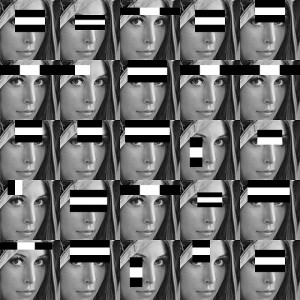
\includegraphics[scale = 0.7]{capitulo_02/figuras_dir/haarcascade.jpg}
\caption{Búsqueda de ``Haar-like features'' en una imagen}
%\label{fig:figura4}
\end{figure}

 







%%%%%%%%%%%%%%%%%%%%% Subsección %%%%%%%%%%%%%%%%%%%%%
\subsection{Calibración de la cámara} \label{s2_2_3}

Para poder llevar a cabo el método de clasificadores en cascada aplicando el algoritmo de Viola-Jones es necesario que 
la imagen no presente distorsión radial, es decir, una imagen que presenta una deformación debido a la lente de la propia cámara que provoca que algunos puntos de la imagen en ciertas zonas se vean mas distanciados que otros puntos de la misma. Dicho de otra forma, esta distorsión provoca que la imagen no se vea en un plano paralelo a la pantalla del ordenador en cuyo caso, todos los puntos de la imagen serían equidistantes a la superficie de la misma. En esta situación, el algoritmo de Viola-Jones no permite conocer con precisión los parámetros de la imagen y por tanto, es necesario corregirla.

En teoría, las lentes convergentes que reciben rayos de luz paralelos al eje óptico hacen converger los rayos en un punto denominado punto focal. Debido a varios motivos como defectos o el fenómeno de difracción que se produce en el material de la lente, puede que no todos estos rayos converjan en el foco de la lente, dando lugar a aberraciones de varios tipos. En este caso, se produce una llamada ``distorsión geométrica'', en la que los bordes de la imagen no son líneas rectas ni están paralelas entre sí. Existen dos tipos de distorsión radial o geométrica: negativa o de barril y positiva o de cojín.

\begin{figure}
\centering
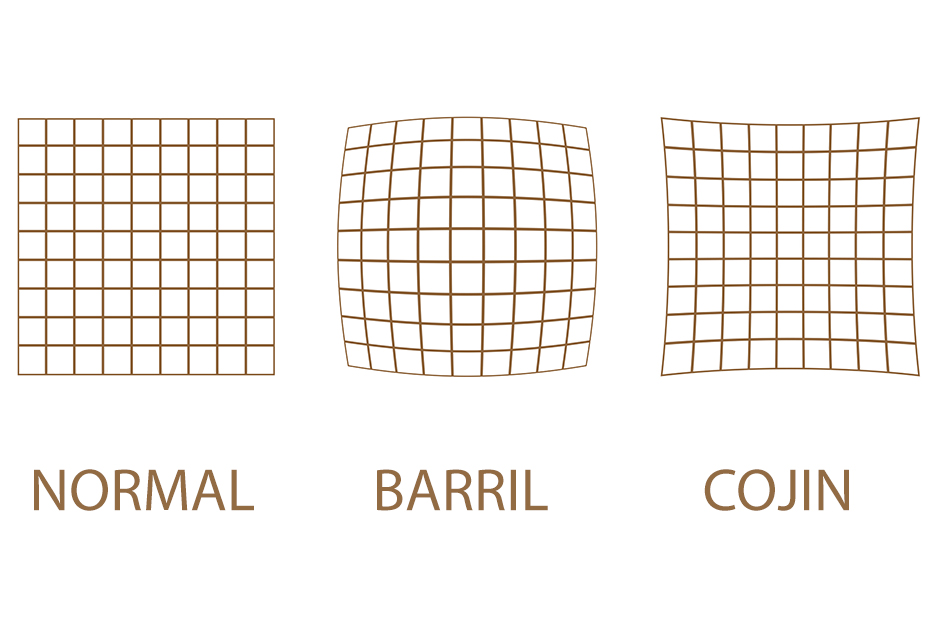
\includegraphics[scale = 0.3]{capitulo_02/figuras_dir/distorsion.jpg}
\caption{Distorsiones geométricas o radiales}
%\label{fig:figura4}
\end{figure}

La librería OpenCV dispone de una serie de algoritmos para la calibración de la cámara. El módulo empleado es ``calib3d''. Para una correcta calibración es necesario obtener los parámetros intrínsecos y extrínsecos de la misma y cuyas distorsiones geométricas estén correctamente corregidas.
Los parámetros intrínsecos son las distancias focales horizontales y verticales de la cámara ($f_x$ y $f_y$), las coordenadas del centro óptico de la imagen ($c_x$ y $c_y$), y las distorsiones radial (k) y longitudinal (p). Los parámetros extrínsecos son aquellos referidos a la posición y la orientación de la cámara respecto al sistema mundo \citep{de2010deteccion}. Los parámetros de traslación se definen como $t_o$ siendo ``o'' el indicador del eje ``x'', ``y'' ó ``z'' y los parámetros de rotación, como $r_{nm}$ siendo ``nm'' los subíndices que indican la posición del parámetro en la matriz donde ``n'' son las filas y ``m'' las columnas.

Matemáticamente, se puede determinar las coordenadas de un punto de la imagen (dos dimensiones) con coordenadas ``u'' y ``v'' partiendo de las coordenadas de su punto homólogo en el espacio (tres dimensiones) de coordenadas ``X'', ``Y'' y ``Z'' respecto un sistema de referencia global o mundo conociendo dos matrices: la matriz de parámetros intrínsecos y la matriz de parámetros extrínsecos.

\begin{equation}
\begin{pmatrix}
u \\
v \\
1 
\end{pmatrix}
=
\begin{pmatrix}
f_x & 0 & c_x\\
0 & f_y & c_y\\
0 & 0 & 1 
\end{pmatrix}
\begin{pmatrix}
r_{11} & r_{12} & r_{13} & t_{x}\\
r_{21} & r_{22} & r_{13} & t_{y}\\
r_{31} & r_{32} & r_{33} & t_{z}
\end{pmatrix}
\begin{pmatrix}
X \\
Y \\
Z \\
1
\end{pmatrix}
\label{matriz}
\end{equation}






Existe una fórmula para obtener las coordenadas ideales de los píxeles conociendo las coordenadas reales y su distancia al centro óptico de la imagen.

\begin{equation}
x_r = x_i + x_i(k_1r^2 + k_2r^4) + 2p_1x_iy_i + p_2(r^2 + 2x_i^2) 
\label{xreal}
\end{equation}
\begin{equation}
y_r = y_i + y_i(k_1r^2 + k_2r^4) + p_1(r^2 + 2y_i^2) + 2p_2x_iy_i
\label{yreal}
\end{equation}

Donde ($x_r$, $y_r$) son las coordenadas reales de los píxeles (de la imagen distorsionada), ($x_i$, $y_i$), las coordenadas ideales (de la imagen sin distorsión) y r, la distancia al centro óptico de la imagen.

A partir de una imagen distorsionada se puede conocer su imagen real y así, evaluar el grado de distorsión que presenta para posteriormente corregirla. El método de corrección de la distorsión sigue un procedimiento matemático más complejo que no es objeto de estudio en este proyecto, sin embargo, de todo esto, lo que es necesario saber es qué se obtiene tras haber efectuado el proceso de calibración\footnote{Véase el capitulo 3.}. Tras realizar el calibrado se obtiene un archivo en formato ``.yml'' que contiene los elementos intrínsecos y extrínsecos mencionados anteriormente en estructuras matriciales y vectoriales: 

\begin{itemize}
    \item Elementos intrínsecos:
    \begin{itemize}
        \item Matriz de la cámara
        \item Matriz de coeficientes de distorsión
    \end{itemize}
    \item Elementos extrínsecos:
    \begin{itemize}
        \item Vector de rotación
        \item Vector de traslación
    \end{itemize}
\end{itemize}

%/////////////////// Subsubsección ///////////////////%
\subsubsection{Método de Zhang}\label{s2_2_3_1}

El método Zhang es el método de calibración que se usa en este proyecto. Se trata de un sistema de calibrado que hace uso de una plantilla bidimensional sobre la que captura coordenadas de los puntos de la misma. A diferencia de otros métodos de calibración, el diseño de la plantilla no requiere especial rigurosidad ni tampoco es necesario que ésta esté fija así como la cámara \citep{viala2008procedimiento}. 

En este método, la plantilla debe cumplir con una serie de características:
\begin{itemize}
    \item Su diseño es parecido al de un tablero de ajedrez. 
    \item Debe ser rígida. De esta forma, se evita que la plantilla se doble y no se pueda efectuar un calibrado correcto.
    \item Las casillas blancas y negras deben mantener las misma dimensiones en todos sus lados, es decir, deben ser perfectamente cuadradas.
    \item Debe ser asimétrica. El número de cuadrados de las filas horizontales debe ser distinto al número de cuadrados de las filas verticales de la plantilla.
    \item El número de cuadrados totales de la plantilla puede variar. Si se pretende conseguir mayor sensibilidad con este algoritmo de calibración, la plantilla puede incorporar mayor número de cuadrados. 
\end{itemize}

\begin{figure}
\centering

\includegraphics[scale = 0.4]{capitulo_02/figuras_dir/CHESSBOARD.jpg}
\caption{Plantilla de calibración estilo tablero de ajedrez}
%\label{fig:figura4}
\end{figure}

El proceso de calibración se resume en los siguientes pasos que serán expuestos con mayor detalle en el capítulo 3:
\begin{itemize}
    \item Realizar al menos diez veces capturas de la plantilla en distintas posiciones. Se dice que en realidad bastaría con tomar dos capturas, sin embargo, en la práctica habría gran cantidad de ruido en las imágenes tomadas.
    \item Cargar las imágenes guardadas en ``.jpg'' e iniciar el proceso de calibración con ``calib3d'' de OpenCV.
    \item Guardar el archivo de calibración resultante del proceso anterior. Este archivo contiene parámetros que pueden ser cargados por los correspondientes programas que hagan uso de la cámara para evitar realizar la calibración cada vez que se necesite ejecutarlo.
\end{itemize}

%/////////////////// Subsubsección ///////////////////%
\subsubsection{Archivo de calibración}\label{s2_2_3_2}

El archivo de calibración contiene elementos que son necesarios para corregir la distorsión radial. Dentro de este archivo se encuentran:
\begin{itemize}
    \item Matriz de la cámara\footnote{Camera\_Matrix es el nombre asignado a la matriz de la cámara en el archivo ``.yml''}: Contiene las distancias focales en el eje ``x'' e ``y'' y el punto central de la imagen ($c_x$,$c_y$). Un ejemplo de su representación en el archivo es la siguiente:
\begin{listing}
\begin{minted}[bgcolor=bg,
               frame=lines,
               framesep=2mm,
               linenos]
               {yaml}
Camera_Matrix: !!opencv-matrix
    rows: 3
    cols: 3
    dt: d
    data: [ 8.1501749606322016e+002, 0., 3.1950000000000000e+002, 0.,
    8.1501749606322016e+002, 2.3950000000000000e+002, 0., 0., 1. ]
\end{minted}
\caption{Matriz de la cámara en el archivo ``MiCam.yml''}
\label{Lis: matrizcamarayml}
\end{listing}
    
    
    \item Matriz de distorsión\footnote{Distortion\_Coefficients es el nombre asignado al vector de coeficientes de distorsión en el archivo ``.yml''}: Contiene los coeficientes de distorsión radial (k) y distorsión longitudinal (p): $k_1$, $k_2$, $p_1$, $p_2$ y $k_3$.  Un ejemplo de su representación en el archivo es la siguiente:
    
\begin{listing}
\begin{minted}[bgcolor=bg,
               frame=lines,
               framesep=2mm,
               linenos]
               {yaml}
Distortion_Coefficients: !!opencv-matrix
    rows: 5
    cols: 1
    dt: d
    data: [ -6.2774279796243893e-002, -1.3722382248069229e+000, 0., 0.,
    1.2887877788299360e+001 ]
\end{minted}
\caption{Coeficientes de distorsión en el archivo ``MiCam.yml''}
\label{Lis: coeficientesyml}
\end{listing}


    \item Vector de rotación\footnote{Rotation\_Vector es el nombre asignado al vector de rotación en el archivo ``.yml''}: Contiene los elementos ``$r_{nm}$'' de la submatriz de rotación de parámetros extrínsecos.
    \item Vector de traslación\footnote{Translation\_Vector es el nombre asignado al vector de traslación en el archivo ``.yml''}: Contiene los elementos ``$t_{x}$'', ``$t_{y}$'' y ``$t_{z}$'' de la submatriz de traslación de parámetros extrínsecos.
    \item Exactitud de calibrado\footnote{Calibrate\_Accuracy es el nombre asignado al número que indica la precisión del calibrado en el archivo ``.yml''}: Indica la exactitud del calibrado. Se considera que una buena calibración tiene un valor de exactitud entre 0 y 1. Cuanto más pequeño sea el número, más precisa ha sido la calibración.
    
\begin{listing}
\begin{minted}[bgcolor=bg,
               frame=lines,
               framesep=2mm,
               linenos]
               {yaml}
    Calibrate_Accuracy: 3.7599675272620409e-001
\end{minted}
\caption{Número de exactitud de calibrado en ``MiCam.yml''}
\label{Lis: numeroyml}
\end{listing}
\end{itemize}





%***************** Subsubsubsección *****************%
%\paragraph{Matriz de la cámara}\label{s2_2_3_2_1}


%***************** Subsubsubsección *****************%
%\paragraph{Coeficientes de distorsión}\label{s2_2_3_2_2}


%***************** Subsubsubsección *****************%
%\paragraph{Vector de rotación}\label{s2_2_3_2_3}







%\newpage
%%%%%%%%%%%%%%%%%%%%%%%%%%%%%%%%%%%%%%%%%%%%%%%%%%%%%%%
%		            	Seccion          			  %
%%%%%%%%%%%%%%%%%%%%%%%%%%%%%%%%%%%%%%%%%%%%%%%%%%%%%%%
\section{Comunicaciones Raspberry Pi - Arduino} \label{s2_3}

%%%%%%%%%%%%%%%%%%%%% Subsección %%%%%%%%%%%%%%%%%%%%%
\subsection{Características generales de la comunicación} \label{s2_3_1}

Una vez que Raspberry Pi haya tomado los eventos de los dispositivos de interfaz humana, es necesario enviarlo al computador correspondiente. Para ello, a cada uno se conecta un microcontrolador Arduino que va a ser el encargado de recibir estos datos. Por tanto, es necesario establecer algún tipo de comunicación entre ambos. Esta comunicación está regida por el modelo ``maestro-esclavo''. Este modelo se caracteriza por:

\begin{itemize}
    \item Existir un único maestro y uno o varios esclavos.
    \item El maestro puede dirigirse a ellos individualmente o colectivamente.
    \item Los esclavos únicamente pueden comunicarse con el maestro.
    \item El maestro se encarga de iniciar el proceso comunicativo, en cambio, los esclavos no pueden.
    \item El maestro se encarga de enviar solicitudes a los esclavos.
\end{itemize}

Raspberry Pi es el encargado de iniciar la comunicación y determinar la dirección IP a la que va a enviar los eventos. Por tanto, se encarga de solicitar o demandar a cada Arduino el ingreso de los datos. Es por ello, por lo que Raspberry Pi actúa como maestro y cada Arduino actúa como esclavo, recibiendo los datos transmitidos por Raspberry Pi. Cada uno de los Arduino tienen asignada una única dirección IP. Debido a que Raspberry Pi envía información a cada uno de forma individual, se establece la comunicación en modo unidifusión ya que de lo contrario, el proyecto carecería de sentido.

En las arquitecturas ``cliente-servidor'', el dispositivo que realiza peticiones es el cliente y el dispositivo que espera y recibe las solicitudes de los clientes, procesa y envía la respuesta es el servidor, por tanto, Raspberry Pi puede ser el cliente de la conexión y Arduino, el servidor.

Para establecer una comunicación Raspberry Pi-Arduino via internet, es necesario elegir el protocolo de transporte de datos: TCP o UDP. El protocolo TCP cuenta con un sistema de envío de datos que garantiza la llegada e integridad de los mismos al destinatario a cambio de sacrificar parte del tiempo debido a la existencia de cierta latencia en el proceso comunicativo. En cambio, sucede lo contrario con el protocolo UDP. Estas características son tratadas a continuación.


%%%%%%%%%%%%%%%%%%%%% Subsección %%%%%%%%%%%%%%%%%%%%%
\subsection{Comunicación TCP} \label{s2_3_2}

TCP deriva de sus siglas ``Transmition Control Protocol''. Este protocolo establece las reglas para la transmisión de información entre dos sistemas a través de redes internet junto con el protocolo IP o ``Internet Protocol''. Ambos protocolos trabajan en distintos niveles expuestos por el modelo OSI\footnote{El modelo OSI o ``Open System Interconnection'' define las etapas que intervienen en un proceso de comunicación. Estas etapas son llamadas niveles o capas: nivel físico, nivel de enlace de datos, nivel de red, nivel de transporte, nivel de sesión, nivel de presentación y nivel de aplicación. Todos ellos ordenados de nivel inferior a superior respectivamente.}. El protocolo TCP trabaja en el nivel de transporte.

La función de TCP consiste en establecer la conexión, enviar los datos y cerrar la conexión. El proceso de comunicación se lleva a cabo mediante la identificación previa de las direcciones IP del emisor y del receptor. Tal y como describe Adrián Estrada \citep{corona2004protocolos}, la dirección IP es ``un número único para cada equipo o ``host'' representado por cuatro cifras separadas por puntos, quedando determinado el 255 como límite [...], con la dirección IP queda identificada la máquina del usuario y la red a la que pertenece''.


El envío de paquetes de datos se realiza asegurando que el receptor reciba los datos sin errores y en el orden correcto.  Esto es debido a que por cada paquete que envía el emisor, debe recibir una señal ACK o ``acknowledgement'' para verificar que el receptor ha recibido los datos. En caso de no recibir esta verificación, el receptor procede a reenviar de nuevo la información. Además, cuenta con una función de suma de verificación o ``checksum'. Este mecanismo otorga al protocolo la capacidad de detectar errores en los datos enviados.

A diferencia del protocolo UDP o ``User Data Protocol'', el protocolo TCP sí garantiza la llegada de los datos y mantiene el orden de llegada con el que se envían.
Este es el principal motivo por el cual para el proyecto se ha escogido este protocolo TCP en lugar del anterior. De esta forma, se consigue mayor fiabilidad en la transmisión de datos ya que con latencia mínima y sin cuellos de botella\footnote{El efecto cuello de botella hace referencia a una acumulación de procesos que se quedan a la espera y no pueden ser atendidos. En este contexto, significa que se envían más datos de los que el servidor puede recibir, acumulándose en el búfer y saturándose hasta que la comunicación se interrumpe.}, se pueden conseguir perfectamente los objetivos marcados que persigue el proyecto para el prototipo de sistema de control visual de equipos propuesto.\par

\begin{figure}
\centering
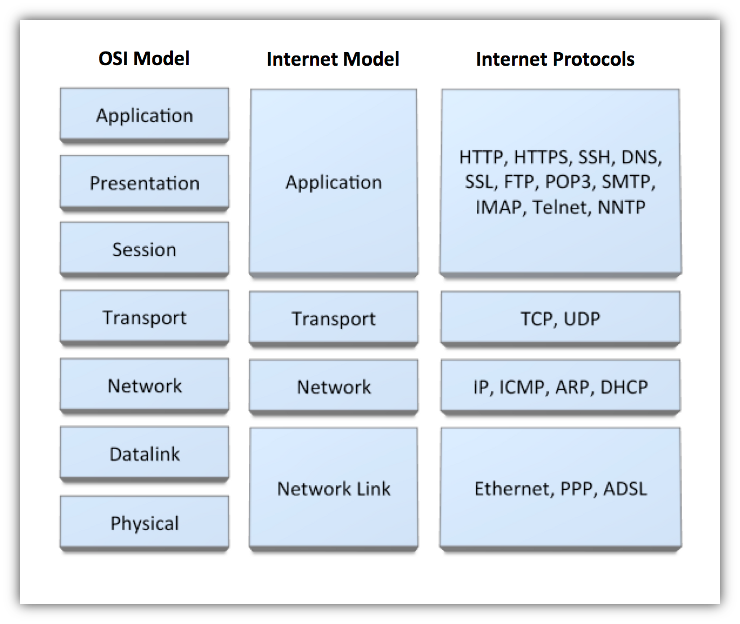
\includegraphics[scale = 0.65]{capitulo_02/figuras_dir/OSI.jpg}
\caption{Niveles del modelo OSI y protocolos de internet aplicados a cada nivel}
%\label{fig:figura4}
\end{figure}









%%%%%%%%%%%%%%%%%%%%%%%%%%%%%%%%%%%%%%%%%%%%%%%%%%%%%%%
%		            	Seccion          			  %
%%%%%%%%%%%%%%%%%%%%%%%%%%%%%%%%%%%%%%%%%%%%%%%%%%%%%%%
\section{Comunicación Arduino - Ethernet Shield} %\label{s2_4}

%%%%%%%%%%%%%%%%%%%%% Subsección %%%%%%%%%%%%%%%%%%%%%
\subsection{Comunicación SPI} %\label{s2_4_1}

SPI es un protocolo de comunicación cuyas siglas proceden de ``Serial Peripheral Interface''. Este protocolo se usa en la conexión Arduino Leonardo con el módulo Ethernet. Se trata de un estándar de comunicación de facto, es decir, ha surgido como un estándar generalmente aceptado y bastante usado hoy en día en muchos de los dispositivos que se fabrican. El hecho de no estar impuesto por un organismo de estandarización provoca que cada fabricante diseñe la interfaz SPI de una forma concreta.

Algunas de las características de este protocolo son:
\begin{itemize}
    \item La comunicación es full-duplex, es decir, el maestro y el esclavo pueden recibir y enviar datos simultáneamente.
    \item Mayor velocidad de transmisión que con el protocolo I2C. En concreto, la velocidad de transmisión es 10 Mbps.
    \item La comunicación es síncrona. Existe una línea de reloj cuyas señales determinan la velocidad con la que se transmite cada bit. 
    \item Distancias cortas. Se emplea para comunicar varios integrados a distancias no superiores a 20 cm.
    \item Es una comunicación en la cual los datos se transmiten en serie (bit a bit).
    \item La interfaz SPI incorpora cuatro hilos:
        \begin{itemize}
            \item {\itshape\bfseries SCLK} o {\itshape\bfseries SCK} (Serial Clock): Es la señal de reloj que genera y emite el maestro o servidor a todos los clientes y que otorga la sincronía característica de esta comunicación.
            \item {\itshape\bfseries MISO} (Master Input, Slave Output): Es la señal de entrada de datos al maestro y de salida de datos del esclavo.
            \item {\itshape\bfseries MOSI} (Master Output, Slave Input): Es la señal de salida del maestro y de entrada de datos al esclavo.
            \item {\itshape\bfseries SS} o {\itshape\bfseries CS} (Chip Select o Slave Select): Es la señal que habilita el integrado que constituye el esclavo de la comunicación. Cuando el maestro quiere enviar y recibir datos con un esclavo, activa SS a nivel bajo. Cuando la comunicación finaliza, de deshabilita cambiando el estado de la señal a nivel alto. Hay tantas líneas SS o CS como esclavos haya (figura \ref{fig: SPI}).
        \end{itemize}
\end{itemize}

Para transmitir un byte completo, es necesario transmitir 8 veces un bit. La transmisión de bits se realiza de la siguiente forma:
\begin{enumerate}
    \item El maestro habilita el esclavo con el que se va a intercambiar información mediante la activación de la línea SS o CS.
    \item El emisor prepara en el registro de salida el byte que se pretende enviar. Si emite el maestro, los bits se transmiten por la línea MOSI. En caso contrario, se transmiten por la línea MISO.
    \item La transmisión se produce bit a bit siguiendo un patrón temporal marcado por la señal cuadrada de reloj generada por el mestro. En cada flanco de bajada, se introduce un bit en MOSI o en MISO.
    \item Por cada flanco de subida, el receptor recoge el bit depositado en la línea y lo introduce en el registro correspondiente.
\end{enumerate}

\begin{figure}
\centering
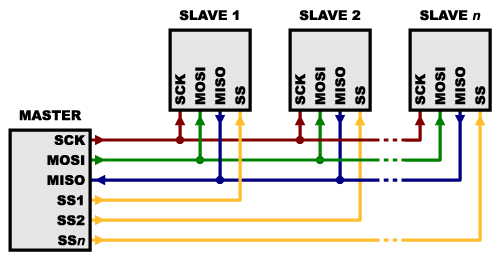
\includegraphics[scale = 0.5]{capitulo_02/figuras_dir/SPI.jpg}
\caption{Conexión SPI del maestro con varios esclavos. Imagen tomada de Prometec: https://www.prometec.net/bus-spi/.}
\label{fig: SPI}
\end{figure}


%%%%%%%%%%%%%%%%%%%%%%%%%%%%%%%%%%%%%%%%%%%%%%%%%%%%%%%
%		            	Seccion          			  %
%%%%%%%%%%%%%%%%%%%%%%%%%%%%%%%%%%%%%%%%%%%%%%%%%%%%%%%
\section{Comunicación Arduino - Equipo} %\label{s2_4}

%%%%%%%%%%%%%%%%%%%%% Subsección %%%%%%%%%%%%%%%%%%%%%
\subsection{Comunicación USB} %\label{s2_4_1}

USB es un protocolo estandarizado. El bus USB o ``Universal Serial Bus'' conecta, comunica y provee alimentación a los dispositivos conectados a él. Este protocolo se usa en la conexión Arduino Leonardo con el correspondiente equipo. Mediante un cable USB 2.0 de extremos tipo A - micro B, se alimenta a Arduino Leonardo y se transmiten los eventos de los dispositivos de interfaz humana al driver del sistema operativo el cual, se encarga de interpretarlos como pulsaciones de teclas y movimientos de ratón mediante un ``sketch'' cargado en el propio microcontrolador que contiene las funciones de simulación. Esto es posible siempre y cuando el sistema operativo reconozca el microcontrolador como un dispositivo HID, es decir, como si estuviera conectado un ratón y un teclado a los puertos USB del computador.

Las características de este protocolo USB 2.0 son:
\begin{itemize}
    \item Alta velocidad: 60 Mbps.
    \item Conexión punto a punto. En un mismo canal o línea se comunican dos nodos. 
    \item Tipología en estrella. Los dispositivos se conectan a un nodo central o concentrador.
    \item Transmisión de datos en serie.
    \item Transmisión asíncrona.
\end{itemize}

Este protocolo utiliza la información que concede el descriptor del dispositivo USB HID. Este descriptor constituye en realidad, un conjunto de bytes en la memoria ROM del computador. Representa información acerca del tamaño de los paquetes de datos, el tipo de paquetes que soporta el dispositivo y la función de cada byte o bit del mismo. 

Tras conectar Arduino Leonardo al computador, este último obtiene el descriptor y lo analiza mediante el driver. Una vez que el sistema operativo reconoce el dispositivo de que se trata, se establece la comunicación y se leen o escriben datos en unos búferes a los cuales, las aplicaciones acceden.

Desde el punto de vista de la capa física del protocolo, existen cuatro líneas principalmente: línea de datos {\itshape D+}, línea de datos {\itshape D-}, línea de alimentación {\itshape Vcc} y línea de masa {\itshape GND}. Cada una de estas líneas se representa en la figura \ref{fig: USB}.

\begin{figure}[H]
\centering
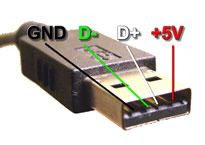
\includegraphics[scale = 0.65]{capitulo_02/figuras_dir/USB.jpg}
\caption{Líneas del bus USB. Imagen tomada de Computación e Informática (blog): http://informmundo.blogspot.com/2010/04/que-llevan-por-dentro-los-cables-usb.html}
\label{fig: USB}
\end{figure}




















%%%%%%%%%%%%%%%%%%%%%%%%%%%%%%%%%%%%%%%%%%%%%%%%%%%%%%%
%		            	Seccion          			  %
%%%%%%%%%%%%%%%%%%%%%%%%%%%%%%%%%%%%%%%%%%%%%%%%%%%%%%%
\section{Programa de selección} \label{s2_4}

%%%%%%%%%%%%%%%%%%%%% Subsección %%%%%%%%%%%%%%%%%%%%%
\subsection{Función} \label{s2_4_1}

El programa de selección permite determinar a qué arduino enviar los eventos recogidos de los periféricos de control. Para ello, previamente se ha desarrollado un programa mediante OpenCV que permite conocer la posición de los ojos con relación a la cara. La finalidad del programa de selección es recoger estos datos de posición y analizarlos adecuadamente.

%%%%%%%%%%%%%%%%%%%%% Subsección %%%%%%%%%%%%%%%%%%%%%
\subsection{Planteamiento del problema} \label{s2_4_2}

Tal y como se describe en el capítulo 3, el programa de detección ocular implementado con OpenCV permite conocer el origen de las regiones cuadradas que delimitan la cara y los ojos. Estos datos son muy importantes para conocer hacia dónde el usuario dirige su mirada y así cederle el control del computador correspondiente. El programa selector debe encargarse de implementar un método que, accediendo a los datos calculados por el programa de seguimiento, sea capaz de obtener el valor de una variable. Este proyecto está diseñado con la posibilidad de haber una pantalla adicional a la pantalla principal que puede situarse a la derecha o a la izquierda, por tanto, esa variable solo puede tener dos valores: ``A'' o ``B''. Cuando el programa selector considere que el control se debe efectuar en el computador principal, el programa devuelve ``A'', en cambio, si considera que el usuario está mirando a una pantalla situada a uno de los dos lados, entonces devuelve ``B''. El programa cliente debe conocer el valor de esta variable para decidir a qué servidor enviar los datos. El procedimiento empleado para desarrollar el programa selector se relata en el siguiente capítulo.






%%%%%%%%%%%%%%%%%%%%%%%%%%%%%%%%%%%%%%%%%%%%%%%%%%%%%%%
%		            	Seccion          			  %
%%%%%%%%%%%%%%%%%%%%%%%%%%%%%%%%%%%%%%%%%%%%%%%%%%%%%%%
\section{Simulación de teclas en Arduino} \label{s2_5}

Cada microcontrolador Arduino debe funcionar como un dispositivo HID conectado al computador para que el sistema funcione como servidor-dispositivo HID al igual que en un sistema de comunicación computador-dispositivo HID convencional. Para ello, es imprescindible que Arduino cuente con un chip ATMega16U2 o ATMega32U2. De esta forma, el computador detecta Arduino como un dispositivo HID y como un microcontrolador simultáneamente.

Mediante un ``sketch'' o programa ``.ino'' que haga uso de las librerías ``keyboard.h'' y ``mouse.h'', los eventos recibidos se simulan como pulsaciones de tecla y movimientos de ratón para que el microcontrolador funcione de la misma forma que un teclado y ratón cualquiera\footnote{Véase el capítulo 3, sección 3.5.}. Esta generación de teclas y movimientos de ratón se produce procesando los ``reports'' de los eventos enviados al equipo vía USB.


%%%%%%%%%%%%%%%%%%%%% Subsección %%%%%%%%%%%%%%%%%%%%%
%\subsection{Teclado} \label{s2_5_1}

%%%%%%%%%%%%%%%%%%%%% Subsección %%%%%%%%%%%%%%%%%%%%%
%\subsection{Ratón} \label{s2_5_2}








%%%%%%%%%%%%%%%%%%%%%%%%%%%%%%%%%%%%%%%%%%%%%%%%%%%%%%%
%		            	Seccion          			  %
%%%%%%%%%%%%%%%%%%%%%%%%%%%%%%%%%%%%%%%%%%%%%%%%%%%%%%%
\section{Funciones útiles de Linux con archivos} \label{s2_7}

%%%%%%%%%%%%%%%%%%%%% Subsección %%%%%%%%%%%%%%%%%%%%%
\subsection{Archivos descriptores: abrir, cerrar, escribir y leer} \label{s2_7_1}

Como ya se ha comentado en la sección 2.1.3.2, los archivos descriptores son números enteros que permite acceder a un conjunto de datos almacenados en una zona de memoria. Existen cuatro funciones básicas que constituyen las ``llamadas al sistema'' que se basan en la apertura y cierre del fichero y en la lectura y escritura del descriptor. Con estas operaciones, se realizan las partes más importantes del proyecto, ya que es necesaria la continua apertura, lectura, escritura y cierre de los drivers de los dispositivos de interfaz humana y de los archivos especiales o FIFO que contienen datos de salida de un programa y de entrada de otro. Todas ellas se describen a continuación, aunque se puede acceder a la información referente a estas operaciones a través del volumen 2 del manual de funciones de llamadas al sistema que incorpora Raspbian:

\begin{itemize}
    \item {\bfseries \itshape open()}: Esta función recibe como argumentos la ruta del fichero y el tipo de apertura (para solo lectura, solo escritura o ambas\footnote{Estas opciones son de tipo ``mode\_t'': O\_RDONLY, O\_WRONLY y O\_RDWR respectivamente}) (``Listing \ref{Lis: apertura}'').
\begin{listing}[H]
\begin{minted}[bgcolor=bg,
               frame=lines,
               framesep=2mm,
               linenos]
               {C}
int open(const char *ruta, mode_t mode);
\end{minted}
\caption{LLamada al sistema de apertura de un archivo}
\label{Lis: apertura}
\end{listing}

    Para abrir el archivo es necesario cargar los archivos cabecera del sistema que se muestran en ``Listing \ref{Lis: cabeceraapertura}''.
\begin{listing}[H]
\begin{minted}[bgcolor=bg,
               frame=lines,
               framesep=2mm,
               linenos]
               {C}
#include <sys/types.h>
#include <sys/stat.h>
#include <fcntl.h>
\end{minted}
\caption{Archivos cabecera del sistema para la apertura del archivo}
\label{Lis: cabeceraapertura}
\end{listing}

    \item {\bfseries \itshape close()}: Esta función recibe como argumento la variable entera que representa al descriptor del archivo abierto previamente (``Listing \ref{Lis: cierre}'').
\begin{listing}[H]
\begin{minted}[bgcolor=bg,
               frame=lines,
               framesep=2mm,
               linenos]
               {C}
int close(int descriptor);
\end{minted}
\caption{LLamada al sistema de cierre de un archivo}
\label{Lis: cierre}
\end{listing}  

    Para cerrar el archivo es necesario cargar el archivo cabecera del sistema que se muestra en ``Listing \ref{Lis: cabeceracierre}''.
\begin{listing}[H]
\begin{minted}[bgcolor=bg,
               frame=lines,
               framesep=2mm,
               linenos]
               {C}
#include <unistd.h>
\end{minted}
\caption{Archivos cabecera del sistema para el cierre del archivo}
\label{Lis: cabeceracierre}
\end{listing}  
    
    \item {\itshape \bfseries write()}: Escribe en el archivo correspondiente a su descriptor el contenido de ``bufer'' hasta n bytes (``Listing \ref{Lis: escritura}'').
\begin{listing}[H]
\begin{minted}[bgcolor=bg,
               frame=lines,
               framesep=2mm,
               linenos]
               {C}
ssize_t write(int descriptor, const void *bufer, size_t n);
\end{minted}
\caption{LLamada al sistema de escritura de un archivo}
\label{Lis: escritura}
\end{listing}    
    
    Para escribir en el archivo es necesario cargar el archivo cabecera del sistema que se muestra en ``Listing \ref{Lis: cabeceraescritura}''.

\begin{listing}[H]
\begin{minted}[bgcolor=bg,
               frame=lines,
               framesep=2mm,
               linenos]
               {C}
#include <unistd.h>
\end{minted}
\caption{Archivo cabecera del sistema para la escritura del archivo}
\label{Lis: cabeceraescritura}
\end{listing} 
    
    \item {\itshape \bfseries read()}: Lee el archivo correspondiente a su descriptor hasta n bytes y lo introduce en ``bufer'' (``Listing \ref{Lis: lectura}'').
\begin{listing}[H]
\begin{minted}[bgcolor=bg,
               frame=lines,
               framesep=2mm,
               linenos]
               {C}
ssize_t read(int descriptor, void *bufer, size_t n);
\end{minted}
\caption{LLamada al sistema de lectura de un archivo}
\label{Lis: lectura}
\end{listing}    

        Para leer el archivo es necesario cargar el archivo cabecera del sistema que se muestra en ``Listing \ref{Lis: cabeceralectura}''.

\begin{listing}[H]
\begin{minted}[bgcolor=bg,
               frame=lines,
               framesep=2mm,
               linenos]
               {C}
#include <unistd.h>
\end{minted}
\caption{Archivo cabecera del sistema para la lectura del archivo}
\label{Lis: cabeceralectura}
\end{listing}
\end{itemize}

       
%%%%%%%%%%%%%%%%%%%%% Subsección %%%%%%%%%%%%%%%%%%%%%
\subsection{Tuberías o pipes} \label{s2_7_2}

Muchos de los programas que se han desarrollado a lo largo del proyecto generan un conjunto de datos que deben ser procesados por otros programas, es decir, la salida de unos programas constituyen las entradas de otros. Esta cadena de procesos es conocida como tubería o en inglés, ``pipeline''. Mediante ese sistema de tuberías se consigue que varios procesos estén comunicados entre sí. Para implementar este método, se usa el sistema de archivos FIFO conocido como ``First Input, First Output'' también llamado tubería con nombre. Con este método de comunicación entre procesos se logra que los datos de salida que entran primero al archivo FIFO son los primeros que salen como entradas de otro proceso. Debido a que los archivos FIFOs implementan tuberías con nombre, el proceso de comunicación solo puede finalizar cuando el proceso receptor ha leído los datos del proceso que los ha escrito. Además, no almacenan datos sino que se encargan de enlazar procesos únicamente.

Los archivos FIFO se pueden crear de cualquiera de las dos formas en el terminal:

\begin{bashcode}
$ mkfifo [opcion]...[nombre]...
\end{bashcode}

Las opciones que incluye son relativas a los modos o permisos del archivo.

\begin{bashcode}
$ mknod [opcion]...[nombre]...[tipo]
\end{bashcode}

El tipo hace referencia a la clase de archivo que se pretende crear: fichero especial de bloques\footnote{Opción ``b''}, fichero especial de caracteres\footnote{Opción ``c'' y ``u''} y FIFO\footnote{Opción ``p'' de pipe o tubería}.
